\documentclass[12pt]{article}
 \usepackage{natbib}
\usepackage[margin=1in]{geometry} 
\usepackage{amsmath,amsthm,amssymb,bm,mathtools}
\usepackage[acronym,shortcuts]{glossaries} % For acronyms
\DeclarePairedDelimiter\bra{\langle}{\rvert}
\DeclarePairedDelimiter\ket{\lvert}{\rangle}
\DeclarePairedDelimiterX\braket[2]{\langle}{\rangle}{#1 \delimsize\vert #2} 
\newcommand{\N}{\mathbb{N}}
\newcommand{\Z}{\mathbb{Z}}
\newcommand{\uvec}[1]{\boldsymbol{\hat{\textbf{#1}}}}

\newtheorem{definition}{Definition}
\newtheorem{thm}{Theorem}
\newtheorem{law}{Law}
\newtheorem{lem}{Lemma}
\newtheorem{cor}{Corollary}
\newtheorem{clm}{Claim}
\usepackage{subcaption,hyperref}
\usepackage[shortlabels]{enumitem}
\hypersetup{
	colorlinks=true, %set true if you want colored links
	linktoc=all,     %set to all if you want both sections and subsections linked
	linkcolor=blue,  %choose some color if you want links to stand out
}

% Acronyms
\newacronym{CE}{CE}{common-envelope}
\newacronym{CEE}{CEE}{common-envelope episode}
\newacronym{RLOF}{RLOF}{Roche-lobe overflow}
\newacronym{BCO}{BCO}{binary compact object}
\newacronym{DNS}{DNS}{double neutron star}
\newacronym{GW}{GW}{gravitational wave}
\newacronym{MS}{MS}{main sequence}
\newacronym{BBH}{BBH}{binary black hole}
\newacronym{DCO}{DCO}{double compact object}
\newacronym{DWD}{DWD}{double white dwarf}
\newacronym{ZAMS}{ZAMS}{zero-age main sequence}
\newacronym{MW}{MW}{Milky Way}
\newacronym{SNR}{SNR}{signal-to-noise ratio}
\newacronym{SKA}{SKA}{Square Kilometre Array}
\newacronym[longplural={supernovae}, plural={SNe}]{SN}{SN}{supernova}

\begin{document}
	
\begin{center}
\Large{\textbf{How Eccentric are LIGO/Virgo Double Neutron Stars?}} \\
\vspace{1cm}
\large{Mike Lau} \\
Last updated: \today
\end{center}

We consider the evolution of a \ac{DNS}, approximated as two point masses in Keplerian orbit, via gravitational radiation reaction to the leading quadrupole order \citep{Peters1964}:
\begin{equation}
\frac{a(e)}{a_0} = \bigg(\frac{e}{e_0}\bigg)^{12/19}
		\frac{1-e_0^2}{1-e^2}
		\bigg( \frac{1+121/304 e^2}{1+121/304e_0^2}\bigg)^{870/2299},
\end{equation}
where the evolution in semi-major axis $a$ is parametrised by the eccentricity $e$, and $a_0$, $e_0$ are the semi-major axis and eccentricity at some point of this evolution. For our purposes, we take them to be the semi-major axis and eccentricity at the formation of the \ac{DNS}, i.e. after the second supernova. We also take $a$ and $e$ to be the respective values when the \ac{DNS} evolves to LIGO/Virgo-sensitive frequencies.

We can safely take the factors $(1+121/304e^2)^{870/2299}$, $(1+121/304e_0^2)^{870/2299}$, and $1-e^2$ to be unity, such that upon rearrangement to make $e$ the subject,
\begin{equation}
\frac{e}{e_0} \approx \bigg(\frac{a}{a_0}\bigg)^{19/12}
\frac{1}{(1-e_0^2)^{19/12}}.
\end{equation}
We find that $e/e_0$ scales as the ratio of the semi-major axis at detection to the semilatus rectum $a_0(1-e_0^2)$ at formation, to the power of $19/12$. We can also recast the equation in terms of the gravitational wave frequency (assumed to be twice the orbital frequency) using $f\propto a^{-3/2}$:
\begin{equation}
\frac{e}{e_0} \approx \bigg(\frac{f_0}{f}\bigg)^{19/18}
\frac{1}{(1-e_0^2)^{19/12}}.
\end{equation}
This shows that the ratio of final to initial eccentricity scales approximately linearly with the ratio of initial to final frequency. The \ac{DNS} eccentricity in the LIGO/Virgo is enhanced by the initial eccentricity $e_0$ in the factor $e_0/(1-e_0^2)^{19/12}$, which is plotted in Fig. \ref{fig:a(e)} (this is Fig. 1 of \cite{Peters1964}). We see that extreme initial eccentricities are required for a significant enhancement; e.g. for $e_0<0.99$, $e_0/(1-e_0^2)^{19/12}$ does not exceed $10^2$.

\begin{figure}
	\centering
	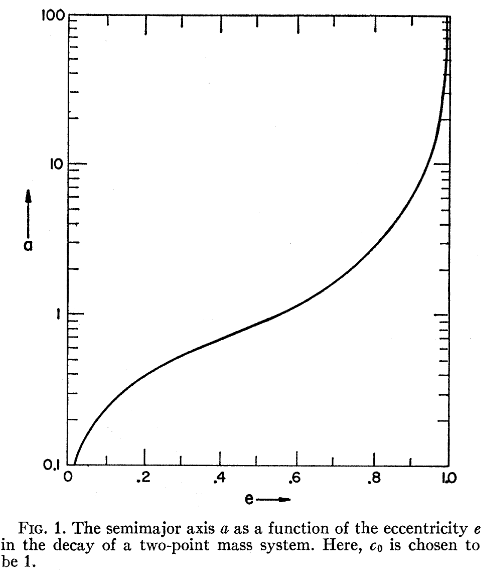
\includegraphics[width=0.5\columnwidth]{Figures/a(e)}
	\caption{$a_0$ vs. $e_0$ \citep{Peters1964}.}
	\label{fig:a(e)}
\end{figure}


\begin{itemize}
	\item For \acp{DNS} being formed with $\sim 1$ day periods ($f_0\sim 10^{-5}$ Hz), observed at a detector lower frequency limit of $f \sim 10$ Hz, $(f_0/f)^{19/18} \sim 10^{-6}$. Therefore if we make the conservative assumption that $e_0<0.99$, the eccentricity $e$ at detection decreases by a factor no less than $10^4$. For $e_0<0.9$, this factor is $10^5$.
	\item If we consider a \ac{DNS} formed via unstable case BB mass transfer, where the additional common-envelope episode circularises the \ac{DNS} at birth to $f_0\sim 10^{-3}$ Hz, this leads to a factor $\sim 100$ enhancement in $e/e_0$. In this case, the eccentricity $e$ at detection decreases by at least a factor of $100$.
\end{itemize}



















\bibliographystyle{apalike}
\bibliography{bibliography.bib}

\end{document}